%%%% -*-Mode: LaTeX -*-

%%
%% Copyright 2007-2019 Elsevier Ltd
%% 
%% This file is part of the 'Elsarticle Bundle'.
%% ---------------------------------------------
%% 
%% It may be distributed under the conditions of the LaTeX Project Public
%% License, either version 1.2 of this license or (at your option) any
%% later version.  The latest version of this license is in
%%    http://www.latex-project.org/lppl.txt
%% and version 1.2 or later is part of all distributions of LaTeX
%% version 1999/12/01 or later.
%% 
%% The list of all files belonging to the 'Elsarticle Bundle' is
%% given in the file `manifest.txt'.
%% 
%% Template article for Elsevier's document class `elsarticle'
%% with harvard style bibliographic references

\documentclass[preprint,12pt,authoryear]{elsarticle}

%% Use the option review to obtain double line spacing
%% \documentclass[authoryear,preprint,review,12pt]{elsarticle}

%% Use the options 1p,twocolumn; 3p; 3p,twocolumn; 5p; or 5p,twocolumn
%% for a journal layout:
%% \documentclass[final,1p,times,authoryear]{elsarticle}
%% \documentclass[final,1p,times,twocolumn,authoryear]{elsarticle}
%% \documentclass[final,3p,times,authoryear]{elsarticle}
%% \documentclass[final,3p,times,twocolumn,authoryear]{elsarticle}
%% \documentclass[final,5p,times,authoryear]{elsarticle}
%% \documentclass[final,5p,times,twocolumn,authoryear]{elsarticle}

%% For including figures, graphicx.sty has been loaded in
%% elsarticle.cls. If you prefer to use the old commands
%% please give \usepackage{epsfig}

%% The amssymb package provides various useful mathematical symbols
\usepackage{amssymb}
\usepackage{color}
\usepackage[normalem]{ulem} % Do not redefine \emph!
\usepackage{hyperref}


\newcommand{\red}{\textcolor{red}}

\newcommand{\mareagalaxy}{\textsf{MaREA4Galaxy}}
\newcommand{\mareaTool}{\textsf{MaREA}}
\newcommand{\clusterTool}{\textsf{Clustering}}
\newcommand{\RASTool}{\textsf{Expression2RAS}}

%% The amsthm package provides extended theorem environments
%% \usepackage{amsthm}

%% The lineno packages adds line numbers. Start line numbering with
%% \begin{linenumbers}, end it with \end{linenumbers}. Or switch it on
%% for the whole article with \linenumbers.
%% \usepackage{lineno}

\journal{Computational and Structural Biotechnology Journal }

\begin{document}

\begin{frontmatter}

%% Title, authors and addresses

%% use the tnoteref command within \title for footnotes;
%% use the tnotetext command for theassociated footnote;
%% use the fnref command within \author or \address for footnotes;
%% use the fntext command for theassociated footnote;
%% use the corref command within \author for corresponding author footnotes;
%% use the cortext command for theassociated footnote;
%% use the ead command for the email address,
%% and the form \ead[url] for the home page:
  
% \title{MaREA4Galaxy: Metabolic Reaction Enrichment Analysis within
% Galaxy\tnoteref{label1}}
  
% \title{\mareagalaxy: a Galaxy tool for metabolic reaction enrichment
% analysis and visualization of RNA-seq data}
  
\title{\textsf{MaREA4Galaxy}: metabolic reaction enrichment analysis
  and visualization of RNA-seq data within Galaxy}


%% use optional labels to link authors explicitly to addresses:
  \author[label3,label1,label2]{Chiara Damiani\corref{cor1}\fnref{eq}}
  \ead{chiara.damiani@unimib.it}
  \author[label1]{Lorenzo Rovida\fnref{eq}}
  \author[label1,label4]{Davide Maspero\fnref{eq}}
  \author[label1]{Irene Sala}
  \author[label1]{Luca Rosato}
  \author[label1]{Marzia Di Filippo}
  \author[label6,label2]{Dario Pescini}
  \author[label5]{Alex Graudenzi}
  \author[label1]{Marco Antoniotti}
  \author[label1,label2]{Giancarlo Mauri}

  \address[label3]{Dept. of Biotechnology and Biosciences,
    Univ. Milano-Bicocca, Milan, Italy}
  \address[label1]{Dept. of Informatics, Systems and Communication,
    Univ. of Milan-Bicocca, Milan, Italy}
  \address[label2]{SYSBIO Centre of Systems Biology, Univ. of
    Milano-Bicocca, Milan, Italy}
  \address[label4]{Fondazione IRCCS Istituto Nazionale dei Tumori,
    Milan, Italy}
  \address[label5]{Institute of Molecular Bioimaging and Physiology of
    the Italian National Research Council (IBFM-CNR), Segrate, Milan,
    Italy}
  \address[label6]{Department of Statistics and Quantitative methods,
    Univ. of Milan-Bicocca, Milan, Italy}

  \cortext[cor1]{Corresponding author}

  \fntext[eq]{equal contributors}
  % \fntext[eq2]{co-senior authors}



  \begin{abstract}
    %% Text of abstract
    
    In this work, we present \mareagalaxy{}, a user-friendly tool that
    allows a user to characterize and to graphically compare groups of
    samples with \red{different \sout{distinct metabolic regulations}
      transcriptional regulation of metabolism}, as estimated from
    cross-sectional RNA-seq data. The tool is available as plug-in for
    the widely-used Galaxy platform for comparative genomics and
    bioinformatics analyses.
    %
    \mareagalaxy~combines \red{ \sout{two} three} modules\red{\sout{:
        the}. The} \red{\RASTool{}} \sout{\mareaTool{} (Metabolic
      Reaction Enrichment Analysis)} module, which, for each reaction
    of a specified set, computes a Reaction Activity Score (RAS) as a
    function of the expression level of genes encoding for the
    \red{associated \sout{reaction}} enzyme\red{. The \mareaTool{}
      (Metabolic Reaction Enrichment Analysis)} module that allows to
    \red{highlight} significant differences \red{in reaction
      activities} between specified groups of samples\red{\sout{;
        the}. The} \clusterTool{} module which employs the RAS
    computed before as a metric for unsupervised clustering of samples
    into distinct metabolic subgroups\red{\sout{. The}; the}
    \clusterTool{} tool provides different clustering techniques and
    implements standard methods to evaluate the goodness of the
    results.

    % integrates into typical genomics analysis within the web-based and
    % well-known platform Galaxy to enable rapid identification and
    % graphical comparison of groups of samples with different metabolic
    % regulations, starting from cross-sectional RNA-seq data.

    % We present \mareagalaxy, a user-friendly system that integrates
    % into typical genomics analysis within the web-based and
    % well-known platform Galaxy to enable rapid identification and
    % graphical comparison of groups of samples with different
    % metabolic regulations, starting from cross-sectional RNA-seq
    % data.
  \end{abstract}

  %% Graphical abstract
  % \begin{graphicalabstract}
  %   \includegraphics{grabs}
  % \end{graphicalabstract}

  %% Research highlights
  % \begin{highlights}
  % \item Research highlight 1
  % \item Research highlight 2
  % \end{highlights}

  \begin{keyword}
    %% keywords here, in the form: keyword \sep keyword
    RNA-seq \sep Metabolism \sep Galaxy \sep Sample stratification \sep
    TCGA

    %% PACS codes here, in the form: \PACS code \sep code

    %% MSC codes here, in the form: \MSC code \sep code
    %% or \MSC[2008] code \sep code (2000 is the default)

  \end{keyword}

\end{frontmatter}


%% \linenumbers

%% main text

\section{Introduction}

In the last \red{\sout{decades} recent years}, life sciences have
witnessed a \red{\sout{change of} renewed} focus
\red{\sout{from genotype towards phenotype} on phenotype level phenomena}. Accordingly, there has been an
increasing attention towards cellular metabolism, which is regarded as
the ultimate level of phenotype, reflecting the response of biological
systems to regulatory and environmental changes. \red{\bfseries MA:
  Vogliamo veramente mettere questa frase in apertura?}

Alteration of metabolic processes plays a pivotal role in many
pathologies, such as cancer, metabolic syndromes, neurodegenerative
diseases \citep{hotamisligil2006inflammation,ward2012metabolic}, as
well as in aging processes \citep{lopez2016metabolic}.

Although quantification of metabolites \red{\sout{is spreading} has
  become more and more feasible}
\citep{Holmes2008}, the difficulty of \textcolor{red}{inferring}
changes in metabolic pathways \red{\sout{from} based on} metabolomics data
\citep{damiani2016linking},
%
\red{\sout{along with the easier access to
    good-quality transcriptomics data,}}
%
\red{\sout{are} is} pushing the need to understand
metabolic alterations \red{\sout{from} by leveraging} gene expression
data.

To this \red{\sout{aim} end}, computational strategies are being
proposed to integrate \textit{--omics} data into metabolic networks
\citep{machado2014systematic,yizhak2015modeling,opdam2017systematic}. Within
this context, we have recently introduced the pipeline
\mareaTool{} % \textsf{MaREA}
(Metabolic Reaction Enrichment Analysis) \citep{marea}
%
\red{\sout{,}. \mareaTool{} \sout{which enables to enlighten}
  characterizes} the metabolic disregulations that distinguish sets of
individuals, by projecting RNA-seq data onto metabolic networks,
without requiring explicit metabolic measurements.

\mareaTool{} computes a Reaction Activity Score (RAS) for each
metabolic reaction and each sample/individual, based on the read count
of the set of genes that encode the catalyzing enzyme(s).
%
The scores are first used as features for cluster analysis and then to
visualize \red{\sout{in a form understandable to life scientists}} the
metabolic disregulations that distinguish the identified
clusters\red{, in a form understandable to life scientists.}

In \citep{marea}, we have demonstrated that \mareaTool{} can
efficiently stratify cancer patients according to their metabolic
activity, as proven by significantly different survival expectancy.
%
Moreover, \mareaTool{} proved to be able to readily capture
metabolic differences between two conditions, such as the properties
that distinguish normal from tumor samples. % \citep{marea}.

The \mareaTool{} pipeline is highly versatile and can be applied to
virtually any study aiming at comparing the metabolism of samples in
different conditions or experimental settings.

In \citep{marea}, we released a MATLAB-based tool that implements the
methodology. However, some technical barriers current limit the
application of the pipeline: MATLAB is a proprietary software and many
life scientists do not have the software licence; moreover, the tool
is not web-based and, therefore, it requires local resources; also,
most life scientists are not familiar with the MATLAB environment.

To overcome these limitations, we present here the freely available
open source web-based tool \mareagalaxy{} which embeds the
\mareaTool{} pipeline within the widely-used platform Galaxy
\citep{galaxy}.
%
\textcolor{red}{Galaxy is a user-friendly web-based workflow system
  that allows biomedical researchers to use computational biology
  tools even without sophisticated \sout{skills in} computer science skills.}
% Galaxy is a user-friendly web-based scientific workflow system that
% has given biomedical researchers without sophisticated understanding
% of computer science access to computational biology
% \citep{galaxy}.

\red{As compared to other user-friendly web-based metabolic network
  visualization tools, such as Escher \citep{king2015escher} or Fame
  \citep{boele2012fame}, which mainly focus on Flux Balance Analysis,
  \mareagalaxy{} specifically enables metabolic reaction enrichment
  analysis of gene expression data which may have been obtained
  directly within the Galaxy environment, for instance by using Galaxy
  tools to produce read counts from raw RNA-seq data. \mareagalaxy{}
  automatically recognizes most common gene nomenclature systems.
  %
  It also enables cluster analysis of samples based on reaction
  activities, as well as on any other features. The cluster analysis
  module implements new functionalities, as compared to the previously
  released MATLAB-based \mareaTool{} tool. New clustering algorithms
  have been included, as well as new instruments for the evaluation of
  clustering goodness and for the selection of the best technique.}

\red{Moreover, \mareagalaxy{} inherits the benefits of Galaxy.  In
  particular, Galaxy allows to build multi-step computational
  analyses. It allows users to upload their own data, as well as to
  interface with public databases, and enables researchers to
  \sout{do} perform the text manipulation required to properly format
  data for analysis without requiring advanced programming skills.
  Galaxy can be downloaded, customized and installed either locally or
  on a dedicated server\sout{, which is provided by many organizations and
  public institutions}. It also provides a comprehensive
  documentation.}

In order to illustrate the functionalities of \mareagalaxy{}, we show a
novel example on real data obtained from The Cancer Genome Atlas
(TCGA) \citep{TCGA}. In particular, we perform an unsupervised cluster
analysis of the gene expression of liver hepatocellular carcinoma
tumors and we analyze the obtained clusters.


\section{Implementation and Availability}

Following the recommendation by Galaxy's \red{\sout{administrators}
  core developers' team}, the back-end
development of \mareagalaxy{} is based on Python and the front-end
development on XML. The interaction between front-end and back-end is
based on the template engine Cheetah. \red{\bfseries MA: Mettere
  almeno un riferimento a Cheetah.}
%
\mareagalaxy{} is \red{\sout{mainly supported by} biolt on top of} the
following libraries: \texttt{lxml}, \texttt{svglib},
\texttt{reportlab}, \texttt{pandas}, \texttt{scipy},
\texttt{python-libsbml}, \texttt{matplotlib}, \texttt{numpy} and
\texttt{scikit-learn} for clustering analysis.

\mareagalaxy{} is stored in a versioned code archive in ToolShed,
\red{\bfseries MA: what is ToolShed?  It must be said.} at:\\
\url{https://toolshed.g2.bx.psu.edu/repos/bimib/marea}.  ToolShed
allows the administrators of the hundreds of public and private Galaxy
servers worldwide to easily install \mareagalaxy, as well as any other
Galaxy utility, into their instances.

Once installed, \mareagalaxy{} appears in the Galaxy toolbar (left bar)
under the name \mareaTool{} (see Figure \ref{fig:screenshot1} for an
example).  A demo of \mareagalaxy{} is available at:
\url{http://bimib.disco.unimib.it:5555}.

\begin{figure}[ht]
  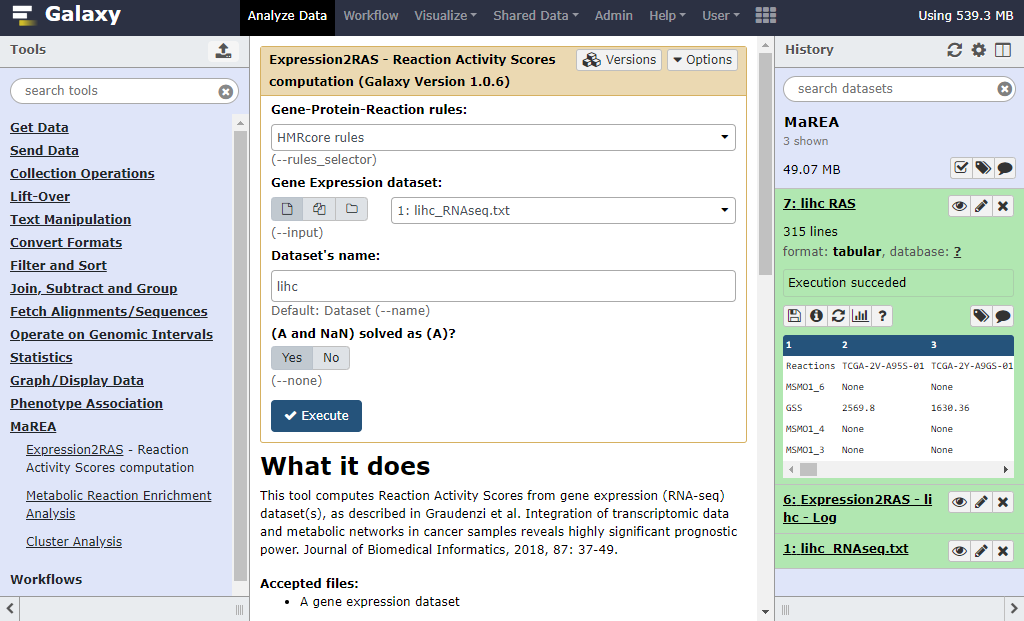
\includegraphics[width=1\textwidth]{figs/screenshot1v2q.png}
  \caption{\red{Screenshot of the \mareagalaxy{} interface. The module
      for RAS computation is illustrated. In particular, the built-in
      (default) HMRcore GPR rules are chosen. \sout{and the input
        format option `RNAseq dataset' have been selected, meaning
        that classification of individuals is not provided. The tool
        will limit to compute the RASs for each individual.} In the
      `add dataset' field there is the RNA-seq dataset which has been
      previously uploaded and that appears in green in the History
      panel on the right.}}
  \label{fig:screenshot1}
\end{figure}

 
\section{Functionalities and Workflow}

\mareagalaxy{} processes datasets stored in the history panel of
Galaxy. These datasets can be uploaded directly from the user's
computer as structured text file by using, e.g., the Galaxy built-in
tool \texttt{Get Data}, or obtained as output of intermediary analyses
performed with other tools.
 
\mareagalaxy{} consists in \red{three \sout{two}} interconnected
modules that may also work independently.
\begin{itemize}
\item \red{The RASs computation module (briefly \RASTool{})}.
\item The metabolic reaction enrichment analysis module
  (\red{\sout{briefly}} \mareaTool{}).
\item The cluster analysis module (\red{\sout{briefly}}
  \clusterTool{}).
\end{itemize}

As better detailed in the following sections, \red{the \RASTool{}
  module computes a RAS for each reaction in each sample. The
  \sout{former} \mareaTool{}} module allows to visualize on a
metabolic map the metabolic reactions that are up- or down- regulated
in different groups of samples \red{either defined \textit{a priori}
  or identified by the \clusterTool{} module}. The \red{\clusterTool{}
  \sout{latter}} module allows to identify sample subgroups (or
clusters) that share similar metabolic properties, ideally by
employing the RAS computed by the \red{\sout{former}} \RASTool{}
module. Any other data can however be used as feature for unsupervised
clustering of \red{samples}\sout{any kind of data}. The metabolic
differences between the \red{\sout{obtained}} clusters \red{thus
  obtained} can, in turn, be analyzed
with the \mareaTool{} module.


\subsection{Computation of Reaction Activity Scores}

The \red{\sout{\mareaTool{}} \RASTool{}} tool selects and extracts
metabolic genes from a gene-expression dataset and, by solving
Gene-Protein-Reaction (GPR) association rules, \red{\bfseries MA: che
  cosa sono queste ``GPR association rules''?} computes a
\emph{Reaction Activity Score} (RAS) for metabolic reactions of
interest, as illustrated in \citep{marea}. The assumption is that
enzyme isoforms contribute additively to the overall activity of a
given reaction, whereas enzyme subunits limit its activity, by
requiring all the components to be present for the reaction to be
catalyzed.
%
\red{\sout{\mareaTool{} then statistically compares the RAS of
    user-defined groups of samples}} \citep{marea}.


\subsubsection{Input}

\red{\sout{\mareagalaxy{}} The \RASTool{} tool
  (Fig.\ref{fig:screenshot1}) takes two \sout{three}} main inputs: 1)
the list of GPRs; 2) the normalized read count of genes from a given
cross-sectional RNA-seq dataset, as, e.g., RPKM (Reads per Kilobase per
Million mapped reads) or TPM (Transcripts Per Kilobase
Million). \red{\sout{and the eventual partition of samples/patients
    into distinct classes; 3) the graphical representation of the
    metabolic network.}}

The first input \red{\sout{reflects the chosen model of metabolic
    network} is a representation of the metabolic model being studied}
and it is basically a dictionary (key-value data structure), which
associates \red{a set of genes} to each metabolic reaction
\red{\sout{a set of genes}}. Both reactions and genes must be defined
by a unique identifier.

Boolean operators AND and OR define the relationship between genes and
enzymes.
%
The AND operator joins genes that encode for different subunits of the
same enzyme, whereas the OR operator joins genes that encode for
isoforms of the same enzyme.

For the user's convenience, two human metabolic network models have
been made directly available within the tool: \textsf{HMRcore} and
\textsf{Recon} 2.2. \textsf{HMRcore} corresponds to the set of GPR
rules included in the core model of central carbon metabolism
introduced in \citep{DiFilippo2016} and was used and curated in
\citep{popFBA,graudenzi2018fbaca,damiani2018integration,marea},
whereas \textsf{Recon} 2.2 \citep{swainston2016recon} is a genome-wide
model encompassing virtually all reactions encoded in human
metabolism.
%
However, the user can also opt to upload any custom metabolic network
model \red{of her/his choice}.

The ID of genes in the dataset must of course coincide with the ID
used in the GPR rules. In case built-in GPRs are used, the following
gene nomenclatures are automatically recognized: HUGO ID, Ensemble ID,
HUGO symbol, Entrez ID.

\red{In case of missing expression value, referred to as NaN (Not a
  Number), for a gene joined with an AND operator in a given GPR rule,
  the user can choose to solve the rule `A AND NaN' as A, or to
  disregard it tout-court (i.e., treated as NaN).}
%% \red{The user can choose whether in case of missing expression
%% value, referred to as NaN (Not a Number), for a gene joined with an
%% AND operator in a given GPR rule, the rule `A and NaN' must be
%% solved as A. Otherwise, the GPR can be disregarded tout-court
%% (i.e., treated as NaN);}


\subsubsection{Output}

\red{\sout{When no partition of samples into classes is specified,
    the}} The tool simply returns as output a dataset reporting
\red{the RAS computed for each sample} for each reaction in the chosen
metabolic network\red{. \sout{the RAS computed for each sample.}} The
RAS dataset is displayed in the History panel.


\subsection{Metabolic Reaction Enrichment Analysis}

\red{The \mareaTool{} tool statistically compares the RAS of
  user-defined groups of samples \citep{marea} and visualizes the
  identified differences.}

\red{According to the user's preference the tool performs the
  following comparisons.
  \begin{itemize}
  \item Pairwise comparison of each group against all other groups.
  \item Comparison of each group against the rest of the samples.
  \item Comparison of each group against a user-defined control group.
  \end{itemize}}


\subsubsection{Input}

\red{\sout{\mareagalaxy} The \mareaTool{}} tool
(Fig.\label{fig:screenshot3}) takes \red{\sout{three main inputs: 1)
    the list of GPRs; 2) the normalized read count of genes from a
    given cross-sectional RNA-seq dataset, as e.g. RPKM (Reads per
    Kilobase per Million mapped reads) or TPM (Transcripts Per
    Kilobase Million) 3)} as main input the Reaction Activity Scores
  of each sample, as computed by the \RASTool{} module and\red{, if
    given,} the eventual partition of samples/patients into distinct
  classes. \sout{2); the graphical representation of the metabolic
    network.}}

The \red{\sout{second} input RAS dataset} can be organized in
\red{\sout{three} two} alternative ways: \red{\sout{1) a unique
    RNA-seq  dataset for all samples/patients; 2)}} 1) two or more
separate \red{\sout{RNA-seq} RAS} datasets, each relative to a
different set of samples/patients; \red{\sout{3)} 2)} a unique
\red{\sout{RNA-seq} RAS} dataset for all samples/patients, plus a file
that associates to each sample its affiliation to a set.

\red{\sout{If a partition of samples into groups is specified,
    \mareaTool\ will compare the RAS of the groups.}} \red{\sout{If
    this is the case, as third} As} (optional) input, the user may
also supply a graphical map of the metabolic network for an efficient
visualization of the analysis outputs. If \red{the} \textsf{HMRcore}
model is chosen, the corresponding map is included within the tool and
does have not to be uploaded. The metabolic map format is a
\texttt{svg} file, reporting metabolites and products of each reaction
linked with an arrow, whose ID matches the name of the reaction in the
GPR file.

\begin{figure}[ht]
  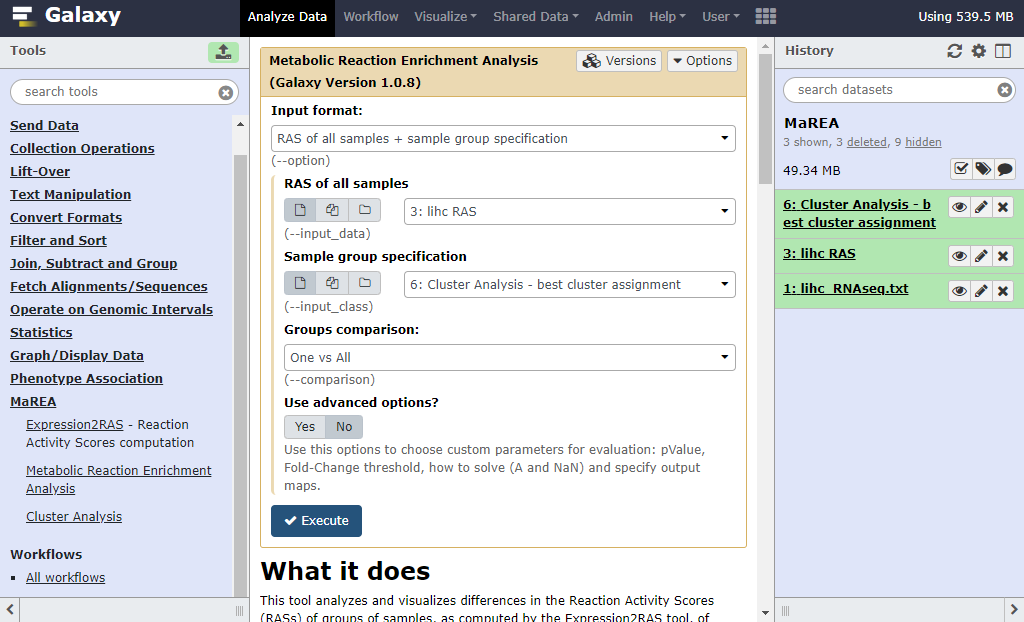
\includegraphics[width=1\textwidth]{figs/screenshot3v2q.png}
  \caption{Screenshot of the \mareagalaxy{} interface. The module for
    metabolic reaction enrichment analysis is illustrated. The input
    format option `RNAseq dataset of all samples + sample group
    specification' has been selected and the best clustering obtained
    with the k-means algorithm in the History has been selected as
    sample group specification.}
  \label{fig:screenshot3}
\end{figure}

\red{\sout{When classes of samples are to be compared (as in the
    example in Figure \ref{fig:screenshot3}),}} The following advanced
options can also be displayed and specified.
\begin{itemize}
\item \red{\sout{ The user can choose whether in case of missing
      expression value, referred to as NaN (Not a Number), for a gene
      joined with an AND operator in a given GPR rule, the rule `A and
      NaN' must be solved as A. Otherwise, the GPR can be disregarded
      tout-court (i.e., treated as NaN).}}
  
\item The P-Value threshold, used for significance Kolmogorov-Smirnov
  (KS) test, to verify whether the distributions of RASs over the
  samples in two sets are significantly different.
  
\item \red{The} threshold of the fold-change between the average RAS of two
  groups. Among the reactions that pass the KS test,  only fold-change
  values larger than the indicated threshold will be visualized on the
  output metabolic map.
  
\item optional outputs to be displayed in the History panel.
\end{itemize}
%
The reader is referred to \citep{marea} for further theoretical
aspects regarding the options above, whereas further technical details
regarding formatting of input files are available in the help section
in Galaxy.


\red{\subsubsection{Output}}

\red{\mareaTool{} returns for each evaluated comparison, a collection
  output in the History including the following items.}

\begin{itemize}
\item A table reporting the fold-change between RASs and p-value of
  the Kolmogorov-Smirnov test.
  
\item The modified metabolic map (whenever supplied as
  input). Reactions up-regulated in the first class as compared to the
  second class  are marked in red, whereas reactions down-regulated in
  the former are marked in blue.
  
  Thickness of arrows is proportional to the fold-change between the
  average RASs of the two classes. Non-Classified reactions, i.e.,
  reactions without information about the corresponding gene-enzyme
  rule, are marked in black.
  %
  Reactions that display a non-significant p-value or a RAS
  fold-change below the threshold are marked in gray color. The pdf of
  the map can directly visualized within Galaxy. The user can also
  download the svg format of the map in order to apply changes;
  
\item A log file, reporting possible warning or error
  messages. Problems that prevent the pipeline's functioning, such as
  wrong format of files, gene ID type not supported or duplicated IDs,
  insufficient number of classes, as well as minor problems, such as
  extra-columns, duplicated labels, missing gene values, or empty
  classes, are properly notified in detail.
\end{itemize}


\subsection{Cluster Analysis}

The \clusterTool{} tool has been conceived to cluster gene expression
data, by using the RAS scores computed by \red{\sout{the tool
    \mareaTool{}} \mareagalaxy{}} as features, given its efficacy in
stratifying cancer patients according to metabolic phenotype, as
demonstrated in \citep{marea}. However, it is suited to cluster
observations in any dataset in which rows indicate different
variables/features and columns different observations.

The \clusterTool{} tool implements three of the main existing algorithms
to cluster data, namely: K-means, agglomerative clustering and DBSCAN
(Density Based Spatial Clustering of Applications with
Noise). Parameters and outputs of the tool are specific of each
algorithm as briefly described in the following.  A screenshot of this
feature of the tool is reported in Figure \ref{fig:screenshot2}.


\subsubsection{K-means}

Given that K-means clustering requires the number of clusters $k$ to
be set by the user, and that it is usually difficult to know the
correct number of clusters \textit{a priori}, the \clusterTool{} tool
allows to \red{evaluate} different values of $k$ and provides standard
methods to estimate the goodness of each clustering in order to choose
the best one. In particular, the elbow plot is generated, which allows
to identify the ``elbow'' (the point of inflection on the curve) as
the best candidate. The tool also generates a \emph{silhouette} plot
for each $k$, which \red{\sout{estimates} reports} \red{\sout{for each
    element}} the cohesion and the separation indexes
\red{\sout{(dissimilarity with elements of other clusters)} of each
  element}\red{\sout{,}. The tool also \sout{and}} computes the
silhouette score of each element, as well as the average silhouette of
each $k$, \red{\sout{to}} returning the $k$ with the best (highest)
silhouette.  The user can specify the minimum and maximum number of
clusters to be evaluated and whether elbow and dendrogram plots must
be generated.

\begin{figure}[ht]
  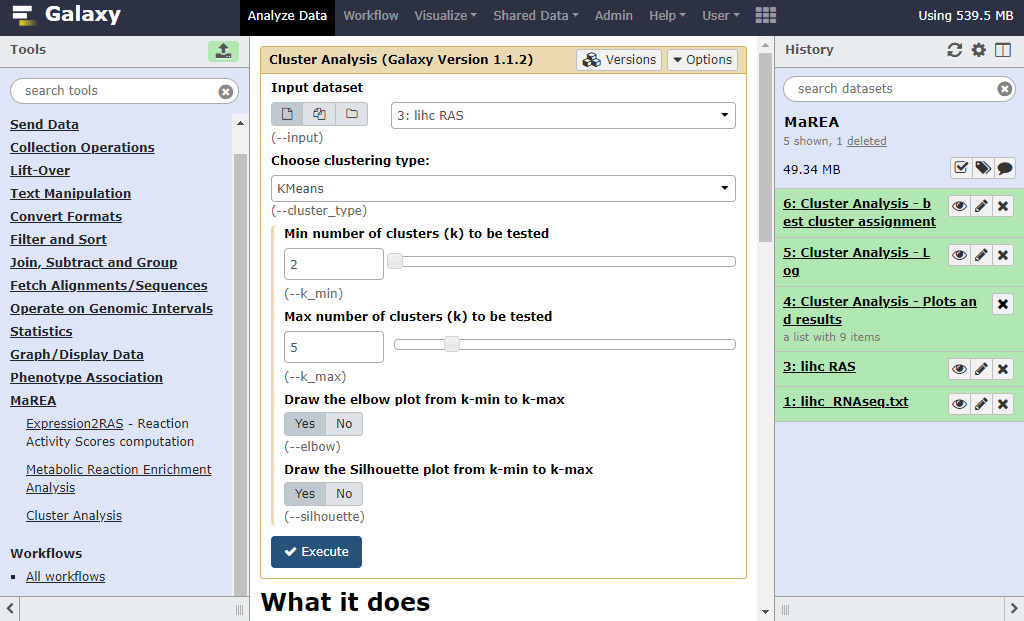
\includegraphics[width=1\textwidth]{figs/screenshot2v2q.png}
  \caption{screenshot of the \mareagalaxy{} interface. The module for
    cluster analysis is illustrated. The RAS computed  by the
    \mareaTool have been selected as input dataset and K-means has
    been chosen as clustering method. 2 to 5 number of clusters will
    be tested. The elbow and silhouette plots will be generated.}
  \label{fig:screenshot2}
\end{figure}


\subsubsection{Agglomerative Clustering}

In the case of agglomerative clustering, the hierarchical output
illustrated by the dendrogram facilitates the choice of the best
clustering. The \clusterTool{} tool returns the set of clusters
obtained when cutting the dendrograms at different points.
%
The user can specify the minimum and maximum number of clusters to be
tested and whether the dendrogram plot must be generated.


\subsubsection{DBSCAN}

The DBSCAN method automatically chooses the number of clusters, based
on parameters that define when a region is to be considered
dense. Custom parameters may be used, namely the maximum distance
between two samples for one to be considered as in the neighborhood of
the other and the number of samples in a neighborhood for a point to
be considered as a core point.


\section{Application Example}

To illustrate \mareagalaxy{} functioning, we show here an example of
application.  We analyze a liver hepatocellular carcinoma RNA-seq
dataset taken from the TCGA pancancer study, including 372 patients.
%
The original data is available at:
\url{http://download.cbioportal.org/blca\_tcga.tar.gz}.
%
For \red{\sout{reviewers'} readers'} convenience, the dataset text
file used for the analyses is also accessible at:
\url{https://tinyurl.com/y3vcustx}.

\red{\sout{With no previous knowledge about the dataset, we aim at
    identifying cohorts of patients with different metabolic
    features.}
The goal of our example is to identify patients' cohorts with
different metabolic features, without assuming any prior knowledge
about the dataset.}
%
\red{\sout{At this aim} To this end}, we first upload our dataset in
the History panel of Galaxy by means of the \red{\sout{tool}}
\texttt{Get Data} \red{tool}. Based on the \textsf{HMRcore} metabolic map, we
then compute the RAS for each reaction in each patient, by means of
\red{\sout{\mareagalaxy{}} \RASTool{}} tool, \red{\sout{by selecting the
    option `RNAseq dataset' and selecting the dataset from the
    history,}} see Figure \ref{fig:screenshot1}.

We then switch to the \clusterTool{} tool and we select as input
dataset the RASs computed before. As a proof of principle, we choose
K-means as clustering algorithm. We test a number of clusters $k$ from
2 to 5, and we indicate that we want to generate both elbow and
silhouette plots for each tested $k$ (see a screenshot of the tool in
Figure \ref{fig:screenshot2}).

The execution of the tool returns the clustering output for each value
of $k$, and indicates as best clustering the one that maximizes the
average silhouette coefficient.
%
In this case, the tools returns $k = 2$ as the best clustering. The
generated elbow and silhouette plots are reported in Figure
\ref{fig:goodness}. It can be noticed that, although we have
identified a good stratification of liver cancer patients, by
qualitative observation of the elbow plot one may also choose $k = 3$
as best clustering.

\begin{figure}[ht]
  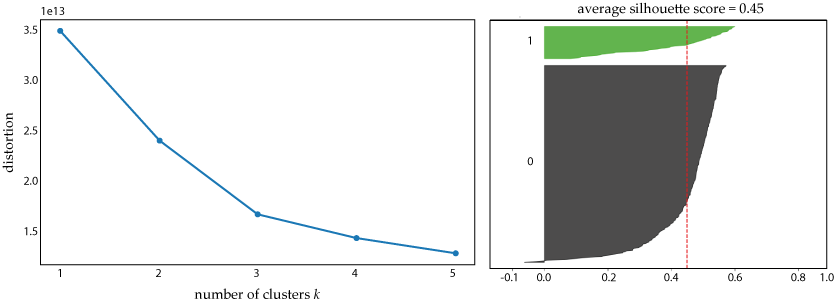
\includegraphics[width=1\textwidth]{figs/goodness.png}
  \caption{Evaluation of clustering goodness by \mareagalaxy{}. Left
    panel: elbow plot generated by the \clusterTool{} module, showing
    an elbow for $k = 2$. Right panel: silhouette plot generated by the
    \clusterTool{} module for $k = 2$, which has been returned as best
    clustering according to the average silhouette score reported in
    the plot's title.}
  \label{fig:goodness}
\end{figure}

Finally, we can use the \mareaTool{} tool to promptly analyze the
differences between the two patients' cohorts. As shown in the
screenshot in Figure \ref{fig:screenshot3}, we select this time the
input format option `RNAseq of all samples + sample group
specification' and we select the best clustering output obtained with
\clusterTool{} as sample group specification file. We flag the option
of generating the pdf map and once we execute the tool we obtain the
map reported in Figure \ref{fig:map}.

\begin{figure}[ht]
  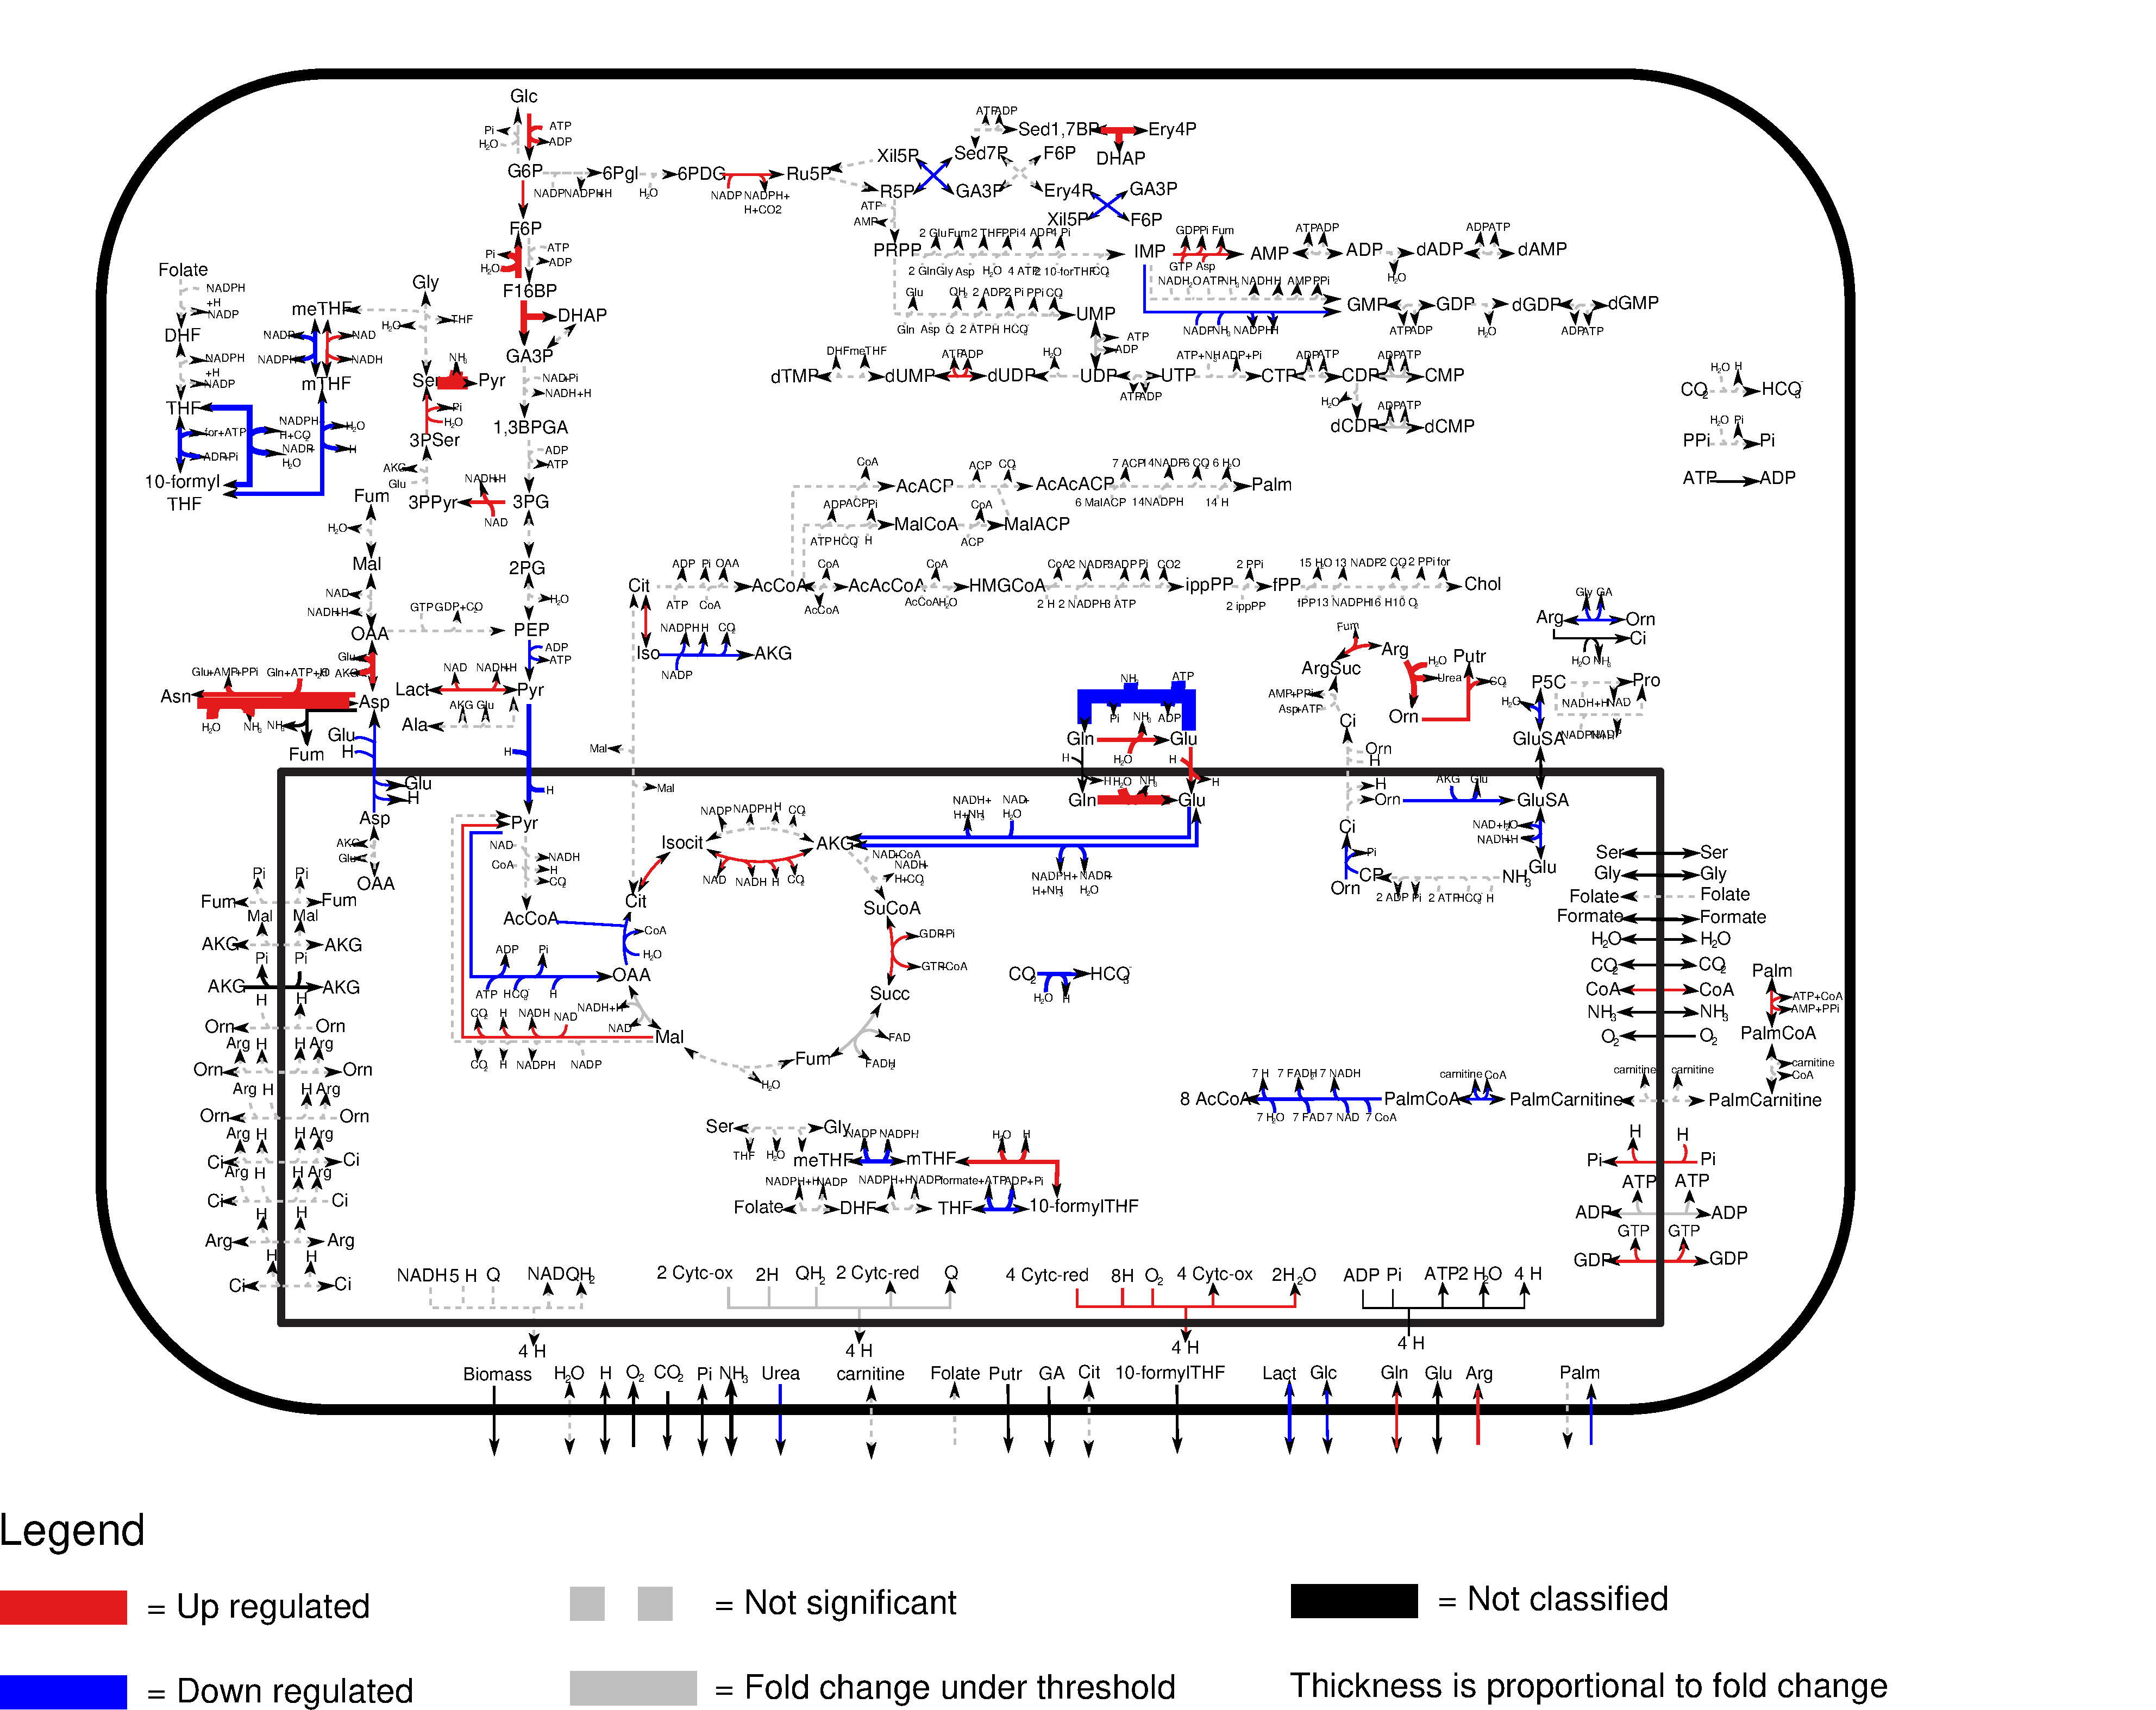
\includegraphics[width=1\textwidth]{figs/map.pdf}
  \caption{Example of metabolic map generated by \mareagalaxy{}. In the
    example, red arrows indicate reactions up-regulated, whereas blue
    arrows reactions down-regulated, in a subgroup of liver
    hepatocellular carcinoma patients. Black arrows refer to reactions
    without information about the corresponding gene-enzyme
    rule. Dashed gray arrows refer to non significant disregulations
    according Kolmogorov-Smirnov test with p-value 0.01. Solid gray
    arrows refer to reactions with a variation lower then 20\%.}
  \label{fig:map}
\end{figure}

Although a few reactions significantly differ between the two cluster,
an \red{\sout{eye that} expert who} is familiar with this classical
representation of central carbon metabolism can immediately notice
(Figure \ref{fig:map}) the main metabolic features that distinguish
the two patients cohorts.

For example, in the first group, the upper glycolytic pathway is
up-regulated, whereas lower glycolysis, upstream of lactate
production, is down-regulated. Lactate production from pyruvate is
instead up-regulated, \red{\sout{clearly}} indicating that pyruvate
production derives from alternative routes, such as from the amino
acid serine derived from glucose. The reactions that go from serine to
pyruvate are indeed up-regulated. Other differences involve the
utilization of glutamine and synthesis of amino acids derived from
glutamine, such as asparagine and aspartate, as well as production of
putrescine and urea in the urea cycle.


\section{Conclusion}

We have shown how with a few intuitive steps, without the need to set
technical parameters, and in a very short time, \mareagalaxy{} enables
to uncover and characterize the differences in metabolic activity
observed in different sample subgroups, as in the case of cancer
patients.

Being empowered by the well-known open and web-based platform Galaxy
for performing accessible, reproducible, and transparent
bioinformatics science, \mareagalaxy{} can support many life
scientists \red{\sout{with} who may have} little knowledge of
computational \red{\sout{sciences} methods \sout{in} for} analyzing
the metabolic variability underlying gene-expression datasets,
\red{\sout{either} no matter whether} collected in their labs or
available in public databases, \red{thus} paving the way to
\red{\sout{tackling} tackle} metabolic plasticity and heterogeneity.

As an example, we have shown a novel application of the \mareaTool{}
pipeline to liver hepatocellular carcinoma and we have identified two
groups with well distinct metabolic features. Investigating the
implications of these differences is out of the scope of this
work. However, it would be interesting to analyze whether the two
groups of patients differ in other aspects, such as their prognosis,
(epi)genomic makeup or regulation of signaling pathways.

A better understanding of the fundamental causes of metabolic
heterogeneity is important for personalised treatment of the many
diseases involving metabolic alterations, as well as for targeted
nutrition recommendations and intervention the field of personalized
nutrition.



%% The Appendices part is started with the command \appendix;
%% appendix sections are then done as normal sections
%% \appendix

%% If you have bibdatabase file and want bibtex to generate the
%% bibitems, please use
%%

\clearpage

\section*{References}

\bibliographystyle{elsarticle-harv} 
\bibliography{marea}


\section*{Acknowledgments}

The institutional financial support to SYSBIO - within the Italian
Roadmap for ESFRI Research Infrastructures - is gratefully
acknowledged. CD and GM received funding from FLAG-ERA grant ITFoC.

%% else use the following coding to input the bibitems directly in the
%% TeX file.

%\begin{thebibliography}{00}

%% \bibitem[Author(year)]{label}
%% Text of bibliographic item

%\bibitem[ ()]{}

%\end{thebibliography}
\end{document}

\endinput

%% Keeping a useful ~ (tilde) here because of idiotic Italian
%% keyboards.

%% End of file `elsarticle-template-harv.tex'.
%% End of file `mareaXgalaxy.tex'.
